\section{Pengembangan Prototype RFID Conveyor Belt dengan Arduino}
Pengembangan Prototype RFID Conveyor Belt ini dilakukan berdasarkan penelitian yang telah ada sebelumnya. Tujuan dari di buatnya pengembangan penelitian ini adalah untuk mengurangi waktu delay pada RFID, dimana pada penelitian sebelumnya waktu delay yang di dapatkan masih terlalu lama
\subsection{Perangkat yang dibutuhkan}
\begin{itemize}
\item PC atau Laptop
\item Software Arduino IDE
\item Arduino Uno + kabel USB Arduino
\item Arduino ethernet + kabel LAN
\item Kabel jumper male-famale secukupnya
\item RGB LED
\item RFID
\item LCD (Liquid Crystal Display)
\item Servo
\item Buzzer
\end{itemize}
\subsection{Kabel Jumper}
Kabel jumper adalah kabel elektrik untuk menghubungkan antar komponen di breadboard tanpa memerlukan solder. Kabel jumper umumnya memiliki connector atau pin di masing-masing ujungnya. Connector untuk menusuk disebut male connector, dan connector untuk ditusuk disebut female connector.kabel jumper dibagi menjadi 3 yaitu :
\begin{enumerate}
\item \textbf{Male to Male} : Kabel ini paling direkomendasikan untuk membuat project elektronika pada sebuah breadboard. Contohnya dapat kita lihat seperti pada gambar \ref{male} 
\begin{figure}[!htbp]
\centering
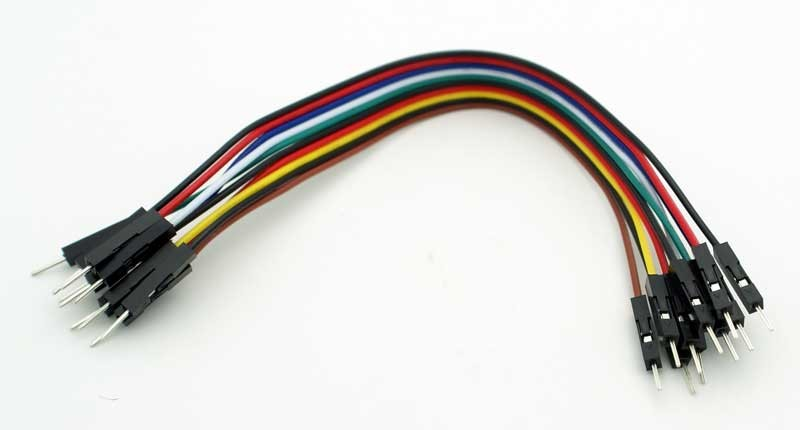
\includegraphics[width=.75\textwidth]{figures/CONV/male.jpg}
\caption{Kabel Jumper Male to Male}\label{fig:male}
\end{figure}
\item \textbf{Male to Female} : Kabel ini memiliki fungsi sebagai penghubung elektronika pada breadboard. Jenis kabel ini memiliki dua header yang berbeda yang menjadikan jenis kabel jumper yang satu ini disebut dengan kabel jumper Male to Female. Contohnya dapat kita lihat seperti pada gambar \ref{mf} 
\begin{figure}[!htbp]
\centering
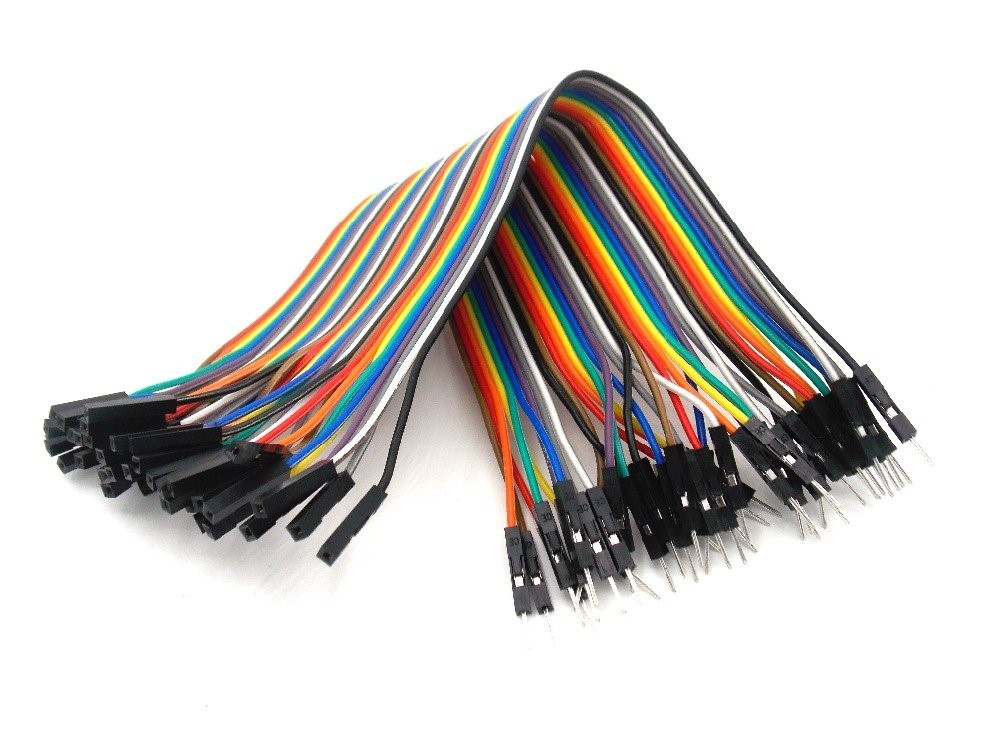
\includegraphics[width=.75\textwidth]{figures/CONV/mf.jpg}
\caption{Kabel Jumper Male to Female}\label{fig:mf}
\end{figure}
\item \textbf{Female to Female} :  Kabel jumper yang satu ini sangat berguna untuk menghubungkan antar module yang memililki header male yang nantinya akan berperan sebagai outputnya. Contohnya dapat kita lihat seperti pada gambar \ref{female} 
\begin{figure}[!htbp]
\centering
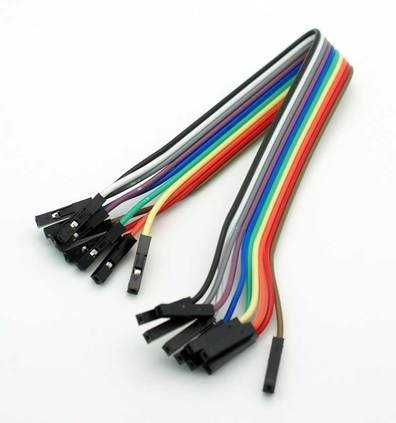
\includegraphics[width=.75\textwidth]{figures/CONV/female.jpg}
\caption{Kabel Jumper Female to Female}\label{fig:female}
\end{figure}
\end{enumerate}

\subsection{RGB LED}
\begin{enumerate}
\item textbf{Perakitan} : Untuk melakukan perakitan pada RGB LED kepada Arduino Uno, kita perlu menghubungkannya dengan menggunakan kabel jumper male to female. Kabel jumper dapat disambungkan seperti pada tabel \ref{table:Perakitan RGB LED}
\begin{table}[h]
\caption{Perakitan}
\centering
\begin{tabular}{|c|c|}
\hline
\textbf{RGB LED}&\textbf{Arduino Uno}\\
\hline
GND&GND\\
\hline
Green&A0\\
\hline
Blue&A1\\
\hline
Red&A2\\
\hline
\end{tabular}
\label{table:Perakitan RGB LED}
\end{table}

\begin{figure}[!htbp]
\centering
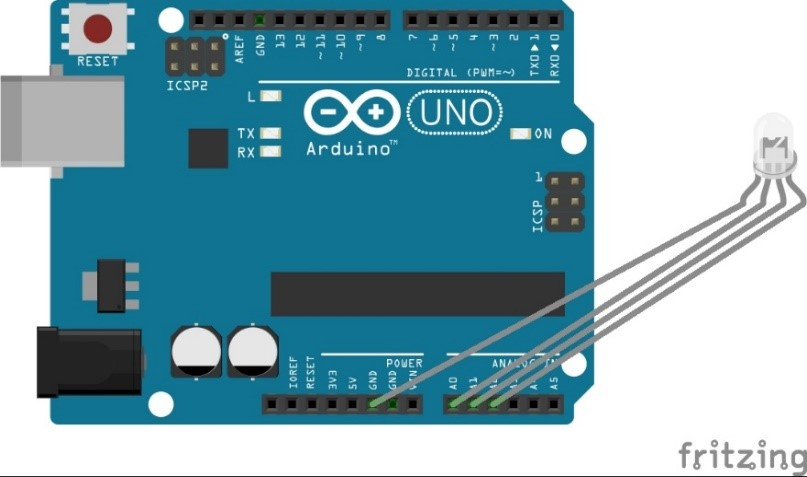
\includegraphics[width=.75\textwidth]{figures/CONV/rgb.jpg}
\caption{Sambungan antara RGB LED dengan Arduino Uno}\label{fig:rgb}
\end{figure}

\item \textbf{Source Kode} : Pertama adalah mendefinikan bahwa di pin A0,A1,A2 adalah pin LED dan membuat semua pin led itu menjadi output yg artinya menyala. Setelah di void loop kita dapat menyalakan lampu dan memberikan delay.
\begin{figure}[!htbp]
\centering
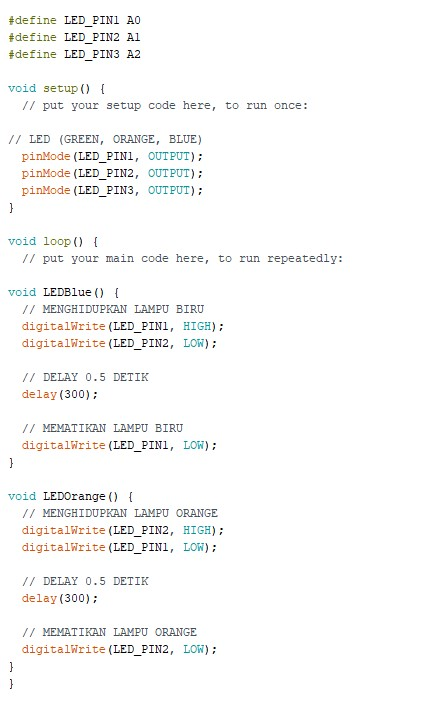
\includegraphics[width=.75\textwidth]{figures/CONV/cov1.jpg}
\caption{Source Code}\label{fig:cov1}
\end{figure}
\end{enumerate}

\subsection{RFID}
\begin{enumerate}
\item \textbf{Perakitan} : Untuk struktur perakitan pada RFID dengan Arduino Uno kita harus menggunakan kabel jumper female to female untuk menghubungkannya. Contohnya dapat kita lihat seperti pada tabel \ref{table:Perakitan RFID}
\begin{table}[h]
\caption{Perakitan}
\centering
\begin{tabular}{|c|c|}
\hline
\textbf{RFID}&\textbf{Arduino Uno}\\
\hline
SDA&Digital 10\\
\hline
SCK&Digital 13\\
\hline
Mosi&Digital 11\\
\hline
Miso&Digital 12\\
\hline
GND&GND\\
\hline
RST&Digital 9\\
\hline
3.3V&3.3V\\
\hline
\end{tabular}
\label{table:Perakitan RFID}
\end{table}

\begin{figure}[!htbp]
\centering
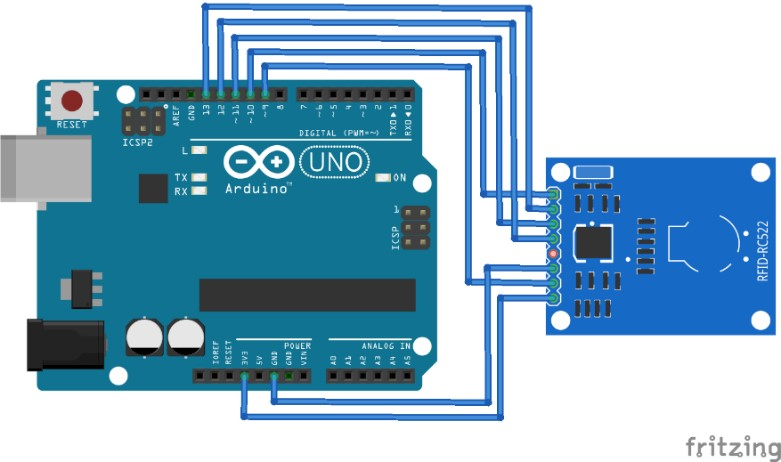
\includegraphics[width=.75\textwidth]{figures/CONV/rfid.jpg}
\caption{Sambungan antara RFID dengan Arduino Uno}\label{fig:rfid}
\end{figure}

\subitem Yang pertama kita lakukan adalah meng-import librarie yaitu SPI,MFRC522, dan Ethernet. SPI berguna untuk mengubungkan lebih dari satu mikrokontroler dimana disini kita menghubungkan Arduino uno dan ethernet, MFRC522 adalah librarie untuk RFID nya, dan yang terkahir adalah librarie untuk Arduino ethernet. Dan selanjutnya kita mendefinisikan alamat ip untuk Arduino ethernet nya yaitu 192.168.8.98, setelah itu kita juga harus mengubah jaringan kita menjadi static menjadi 192.168.8.99 agar data nya dapat terkirim ke com kita.

\begin{figure}[!htbp]
\centering
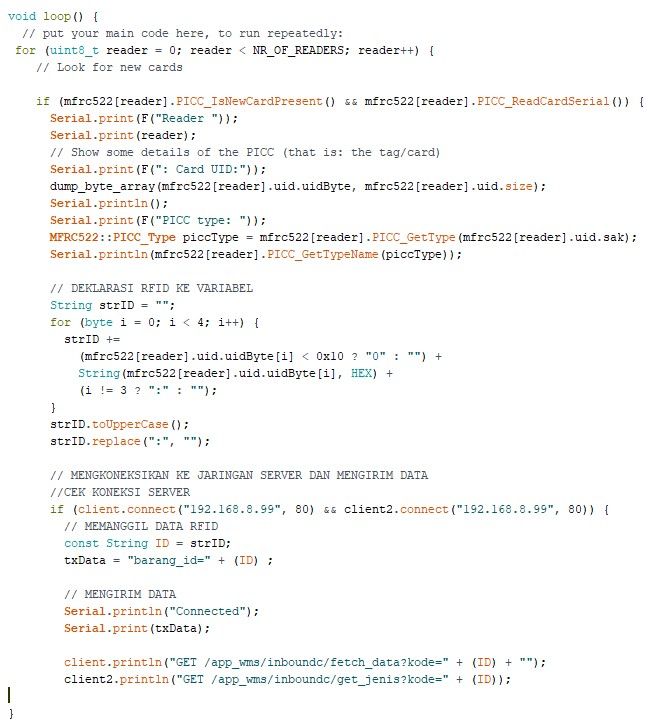
\includegraphics[width=.75\textwidth]{figures/CONV/cov2.jpg}
\caption{Code Void Loop}\label{fig:cov2}
\end{figure}

\subitem Gambar \ref{fig:2} adalah void loop yg dimana ini akan di jalakan terus menerus, ini adalah codingan untuk rfid, artinya adalah Reader mana yang telah membaca si tag dan apa kode si tag tersebut dan selanjut nya kode tersebut akan di kirim melalui ip yang telah di setting sebelum nya.
\end{enumerate}

\section{LCD}
\begin{enumerate}
\begin{table}[h]
\caption{Perakitan}
\centering
\begin{tabular}{|c|c|}
\hline
\textbf{LCD}&\textbf{Arduino Uno}\\
\hline
GND&GND\\
\hline
VCC&5 V\\
\hline
SDA&A4\\
\hline
SCL&A5\\
\hline
\end{tabular}
\label{table:Perakitan LCD}
\end{table}
\item Pemasangan kabel jumper yang digunakan adalah kabe male to male seperti pada gambar \ref{fig:lcd}

\begin{figure}[!htbp]
\centering
\includegraphics[width=.75\textwidth]{figures/CONV/lcd.jpg}
\caption{Kabel jumper pada LCD dan Arduino}\label{fig:lcd}
\end{figure}



\end{enumerate}